\documentclass[12pt]{article}
\RequirePackage{amsthm,amsmath,amsbsy,amsfonts}
\usepackage{graphicx}
%\usepackage{enumerate}
\usepackage{natbib}
\usepackage{url} % not crucial - just used below for the URL 
\usepackage{placeins}

%\pdfminorversion=4
% NOTE: To produce blinded version, replace "0" with "1" below.
\newcommand{\blind}{0}

% DON'T change margins - should be 1 inch all around.
\addtolength{\oddsidemargin}{-.5in}%
\addtolength{\evensidemargin}{-.5in}%
\addtolength{\textwidth}{1in}%
\addtolength{\textheight}{1.3in}%
\addtolength{\topmargin}{-.8in}%


\begin{document}
	\title{Supplementary Material}	 
	
	\section{ADMM details}
	We first re-parameterize $\phi_j = y-\theta_j$ so the problem is
	\begin{equation}
	\text{minimize } \rho_\tau(\phi) + \lambda||D^{(k)}(y-\phi)||_1\\
	\end{equation}
	
	
	We further divide $\phi$ order to solve smaller problems: Defining
	\begin{align}
	&\phi_1 = (\phi_{11}, \phi_{12})\\
	&\phi_2 = (\phi_{21}, \phi_{22}, \phi_{23})\\
	&\phi_3 = (\phi_{31}, \phi_{32})\\
	&\phi = (\phi_{11}, \phi_{12}=\phi_{21}, \phi_{22}, \phi_{23}=\phi_{31}, \phi_{32}) \\
	\end{align}
	Dividing $y$ similarly, the problem then becomes 
	\begin{align}
	&\text{minimize } \sum_{i=1}^3 \rho_\tau(\phi_i) + \lambda||D^{(k)}(y_i-\phi_i)||_1\\
	&\text{subject to: } \phi_{12}=\phi_{21}, ~~ \phi_{23}=\phi_{31}\\
	\end{align}
	We can further simplify by defining 
	\begin{align}
	&\overline{\phi} = (\phi_{11}, \frac{\phi_{12}+\phi_{21}}{2}, \phi_{22}, \frac{\phi_{23}+\phi_{31}}{2}, \phi_{32}) \\
	&\overline{\phi_1} = (\phi_{11}, \frac{\phi_{12}+\phi_{21}}{2})\\
	&\overline{\phi_2} = ( \frac{\phi_{12}+\phi_{21}}{2}, \phi_{22}, \frac{\phi_{23}+\phi_{31}}{2})\\
	&\overline{\phi_3} = (\frac{\phi_{23}+\phi_{31}}{2}, \phi_{32})
	\end{align}
	so the problem becomes
	\begin{align}
	&\text{minimize } \sum_{i=1}^3 \rho_\tau(\phi_i) + \lambda||D^{(k)}(y_i-\phi_i)||_1\\
	&\text{subject to: } \phi_{i}=\overline{\phi_i}\\
	\end{align}
	The augmented Lagrangian for this problem is 
	\begin{align}
	&L_\gamma(\phi_1,\phi_2, \phi_3, \overline{\phi_1}, \overline{\phi_2}, \overline{\phi_3}, \omega) = \\
	&\sum_{i=1}^3 \rho_\tau(\phi_i) + \lambda||D^{(k)}(y_i-\phi_i)||_1 + \omega_i^T(\phi_i - \overline{\phi_i}) + \frac{\gamma}{2}||\phi_i - \overline{\phi_i}||_2^2
	\end{align}
	The ADMM updates are then given by
	\begin{align}
	&\phi_i^{k+1} = \arg\min_{\phi_i}\rho_\tau(\phi_i) + \lambda||D^{(k)}(y_i-\phi_i)||_1 + \omega_i^{kT}(\phi_i - \overline{\phi_i}^k) + \frac{\gamma}{2}||\phi_i - \overline{\phi_i}^k||_2^2\\
	&\omega_i^{k+1} = \omega_i^{k} + \gamma(\phi_i^{k+1} - \overline{\phi_i}^{k+1})
	\end{align}
	The $\phi_i$ updates can be obtained using a quadratic program solver such as Gurobi and can be obtained in parallel. 
	
	\section{Simulation Metrics}
	
	\begin{figure}[h!]
		\caption{F1 score by threshold, data size, and method (1 is best 0 is worst).}
		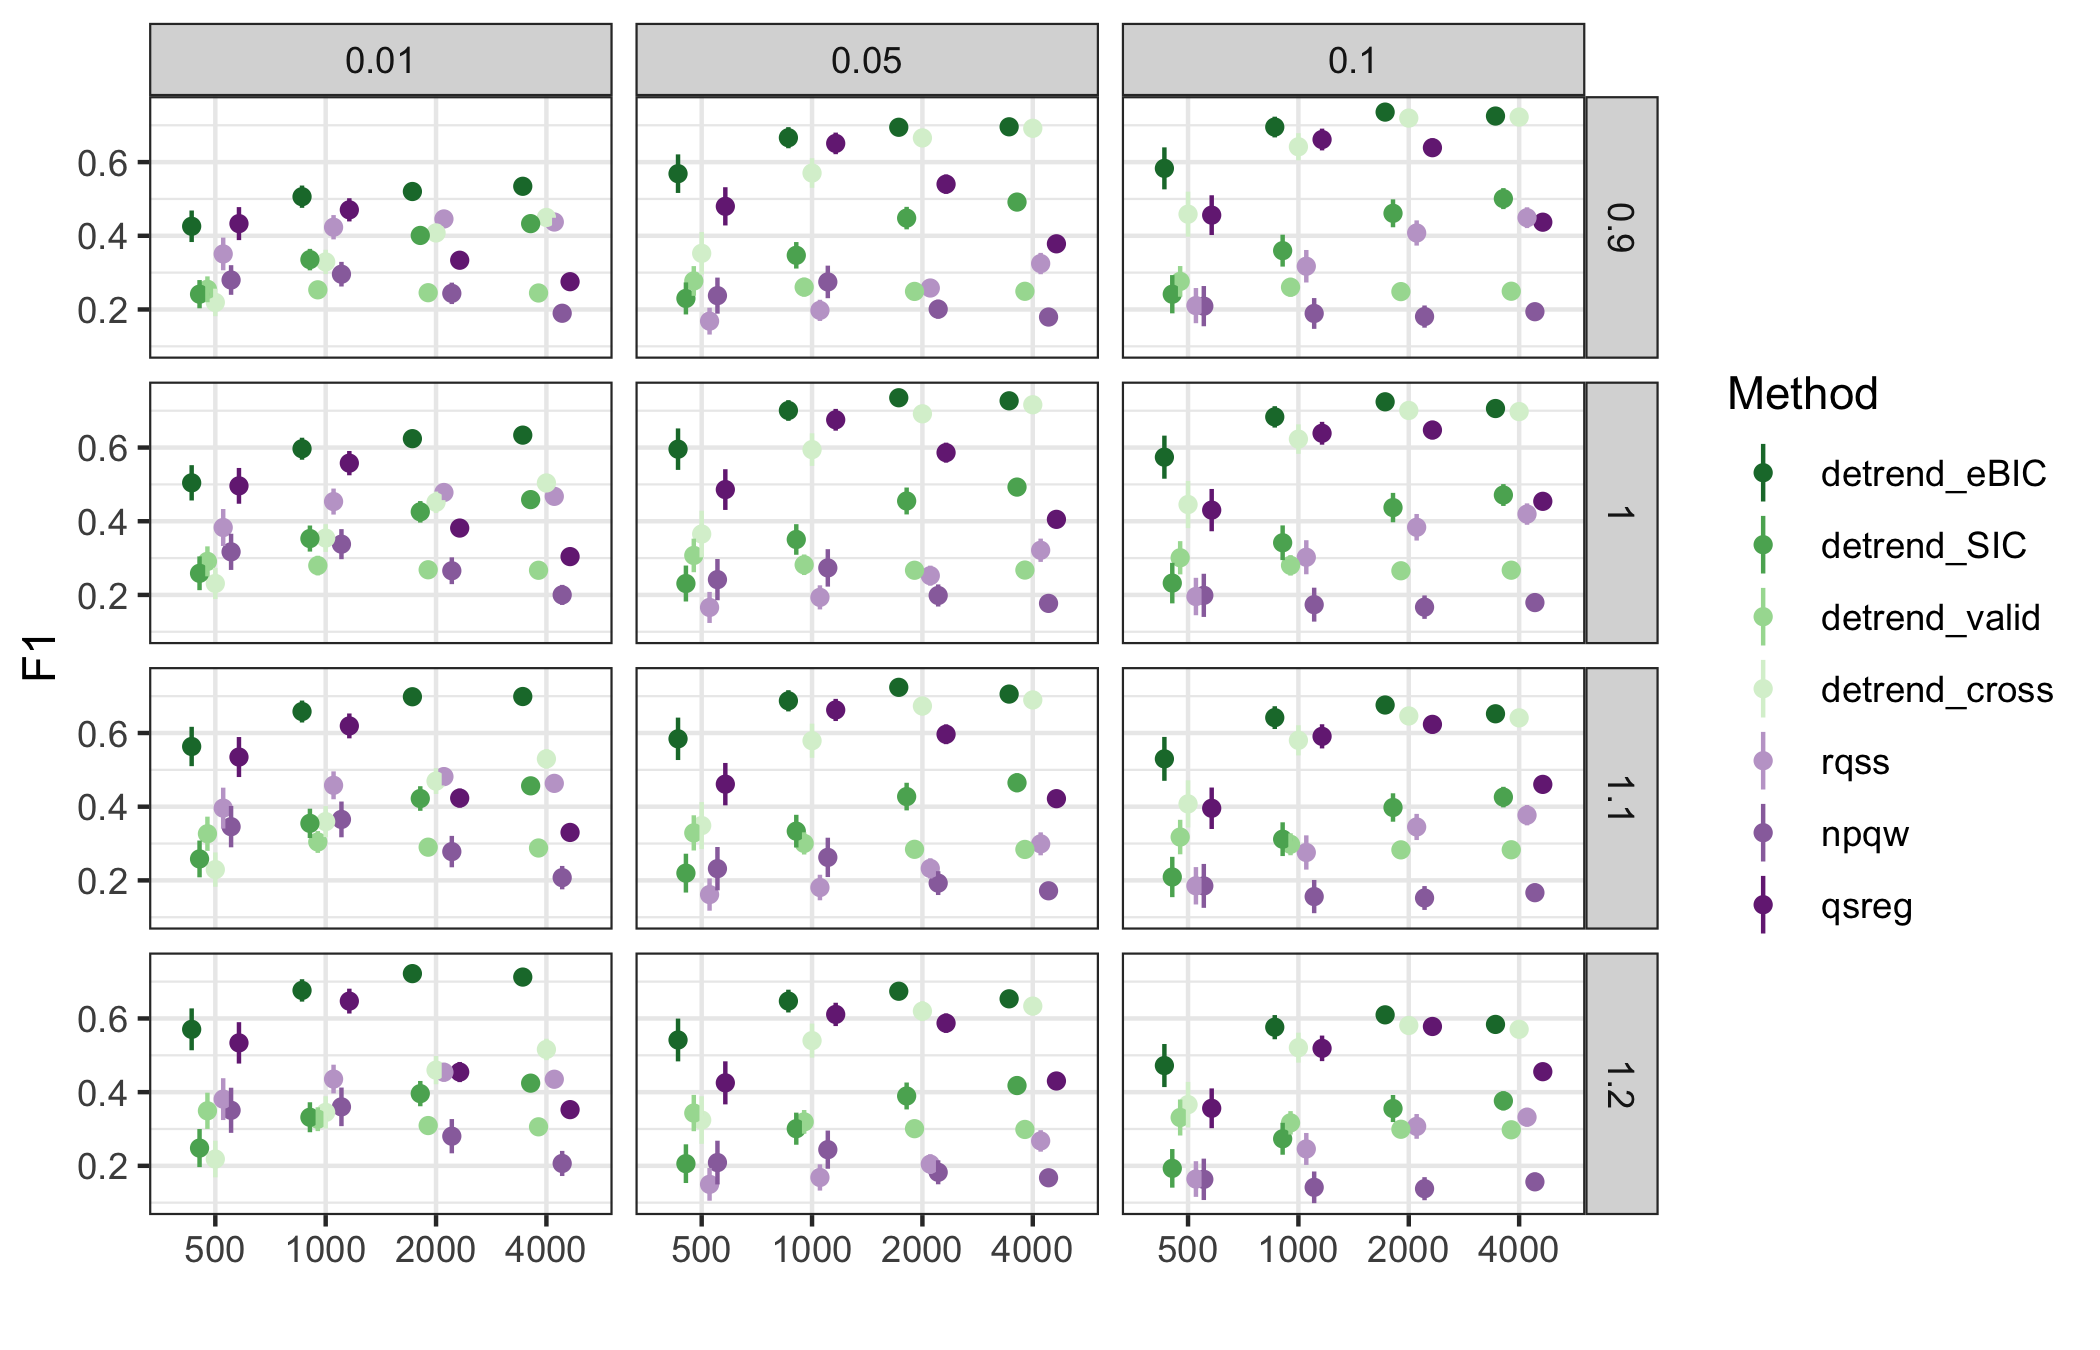
\includegraphics[width = \linewidth]{Figures/peaks_F1.png}
	\end{figure}
	
	\begin{figure}[h!]
		\caption{Precision by threshold, data size, and method (true positive over true positives + false positives).}
		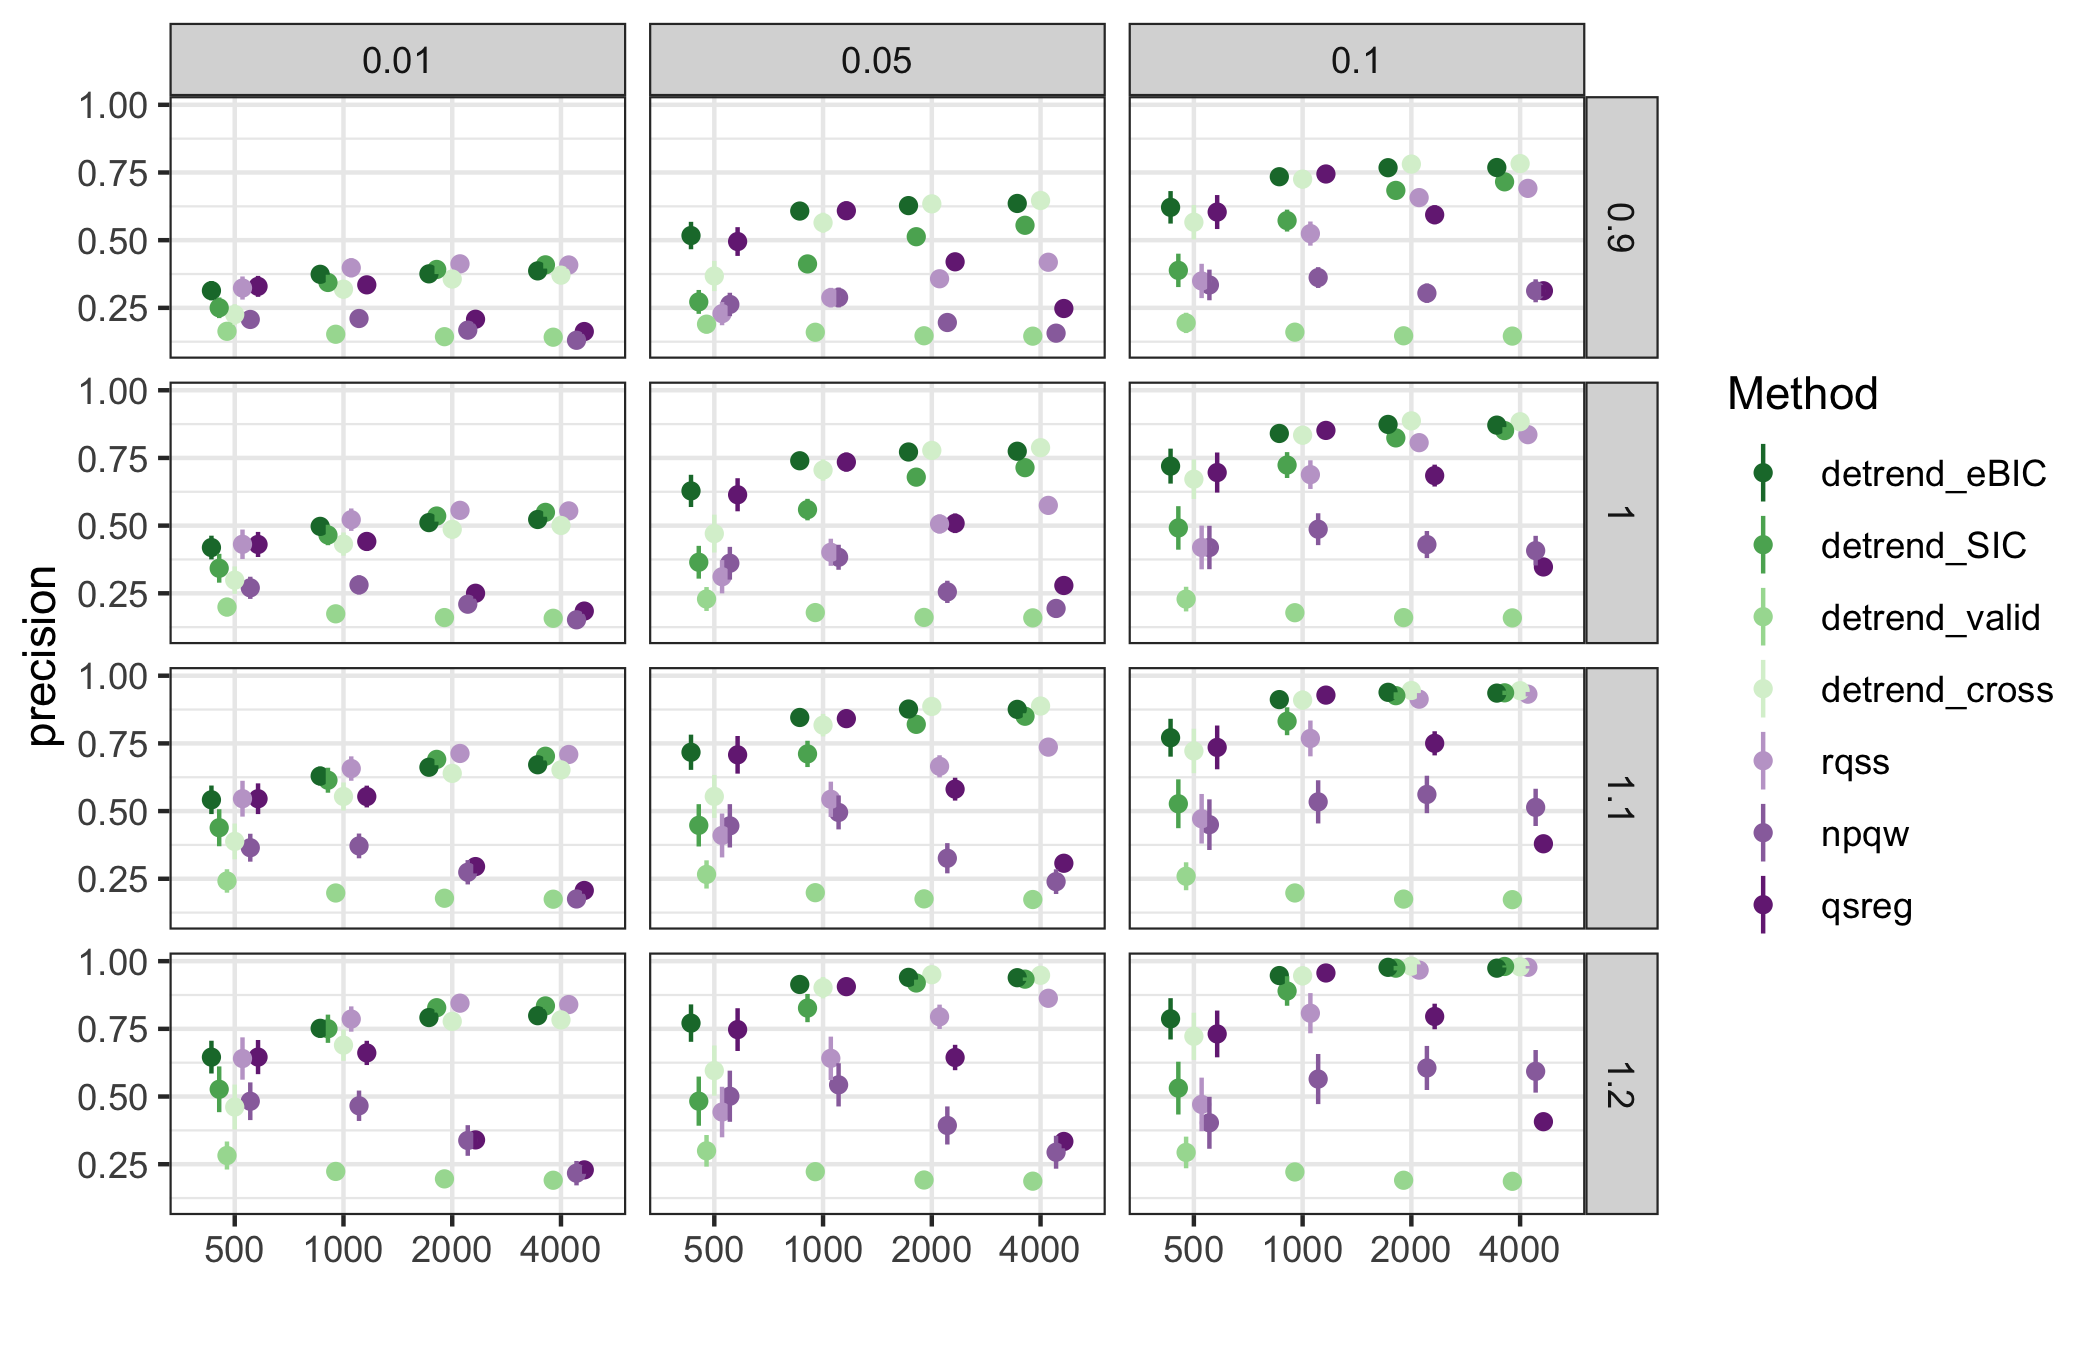
\includegraphics[width = \linewidth]{Figures/peaks_precision.png}
	\end{figure}
	
	\begin{figure}[h!]
		\caption{Recall by threshold, data size, and method (true positive over true positives + false negatives).}
		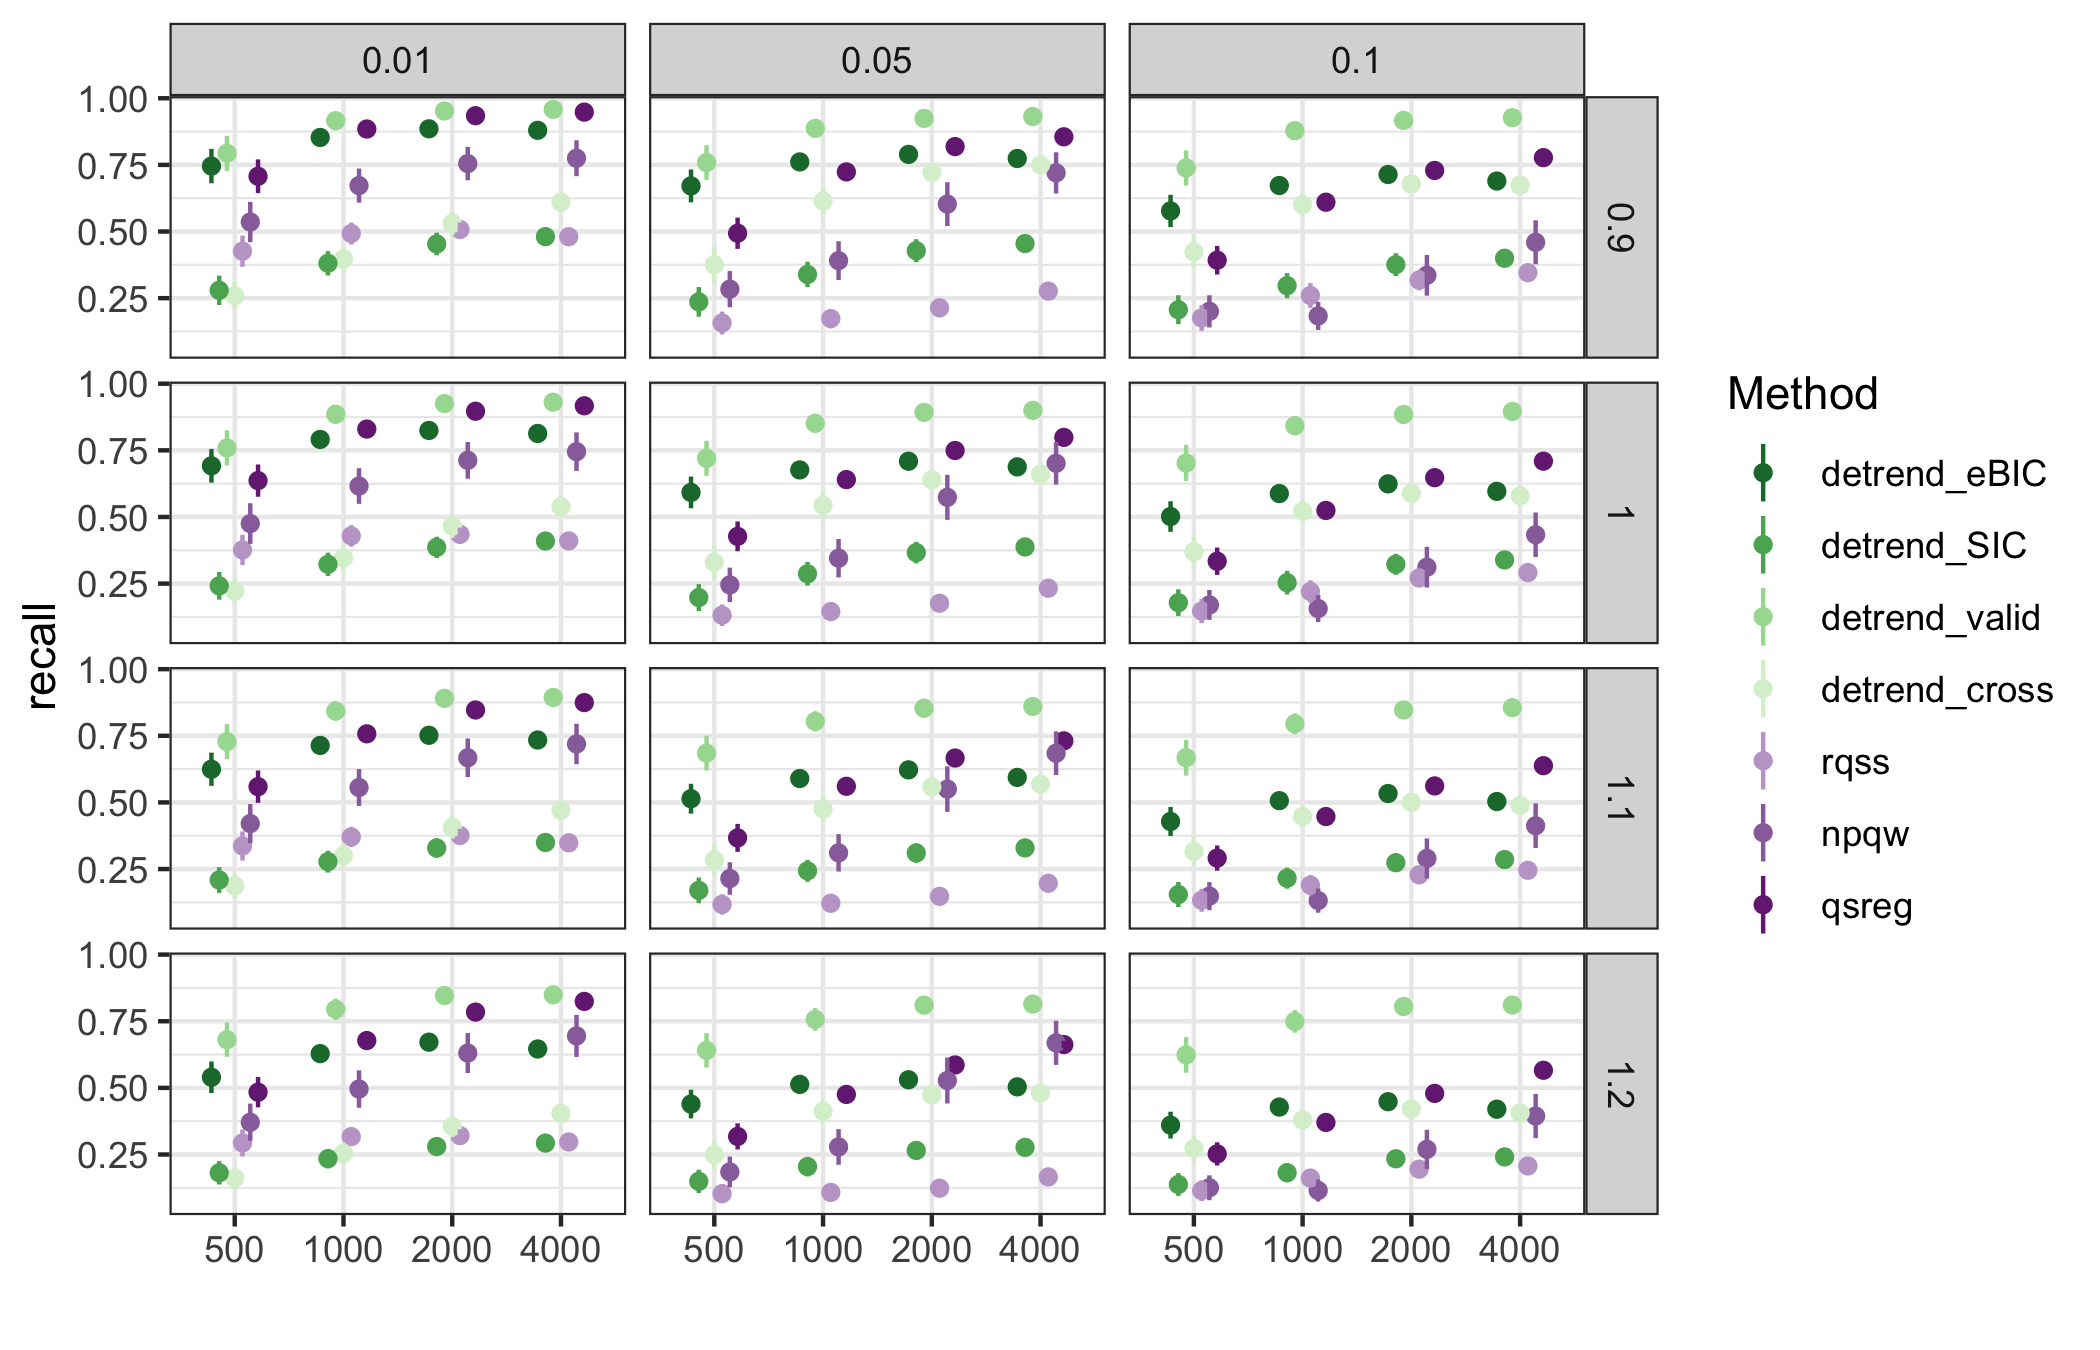
\includegraphics[width = \linewidth]{Figures/peaks_recall.png}
	\end{figure}
	
	\begin{figure}[h!]
		\caption{Miss-classification rates by threshold, data size, and method, values above the upper limit (npqw) not shown.}
		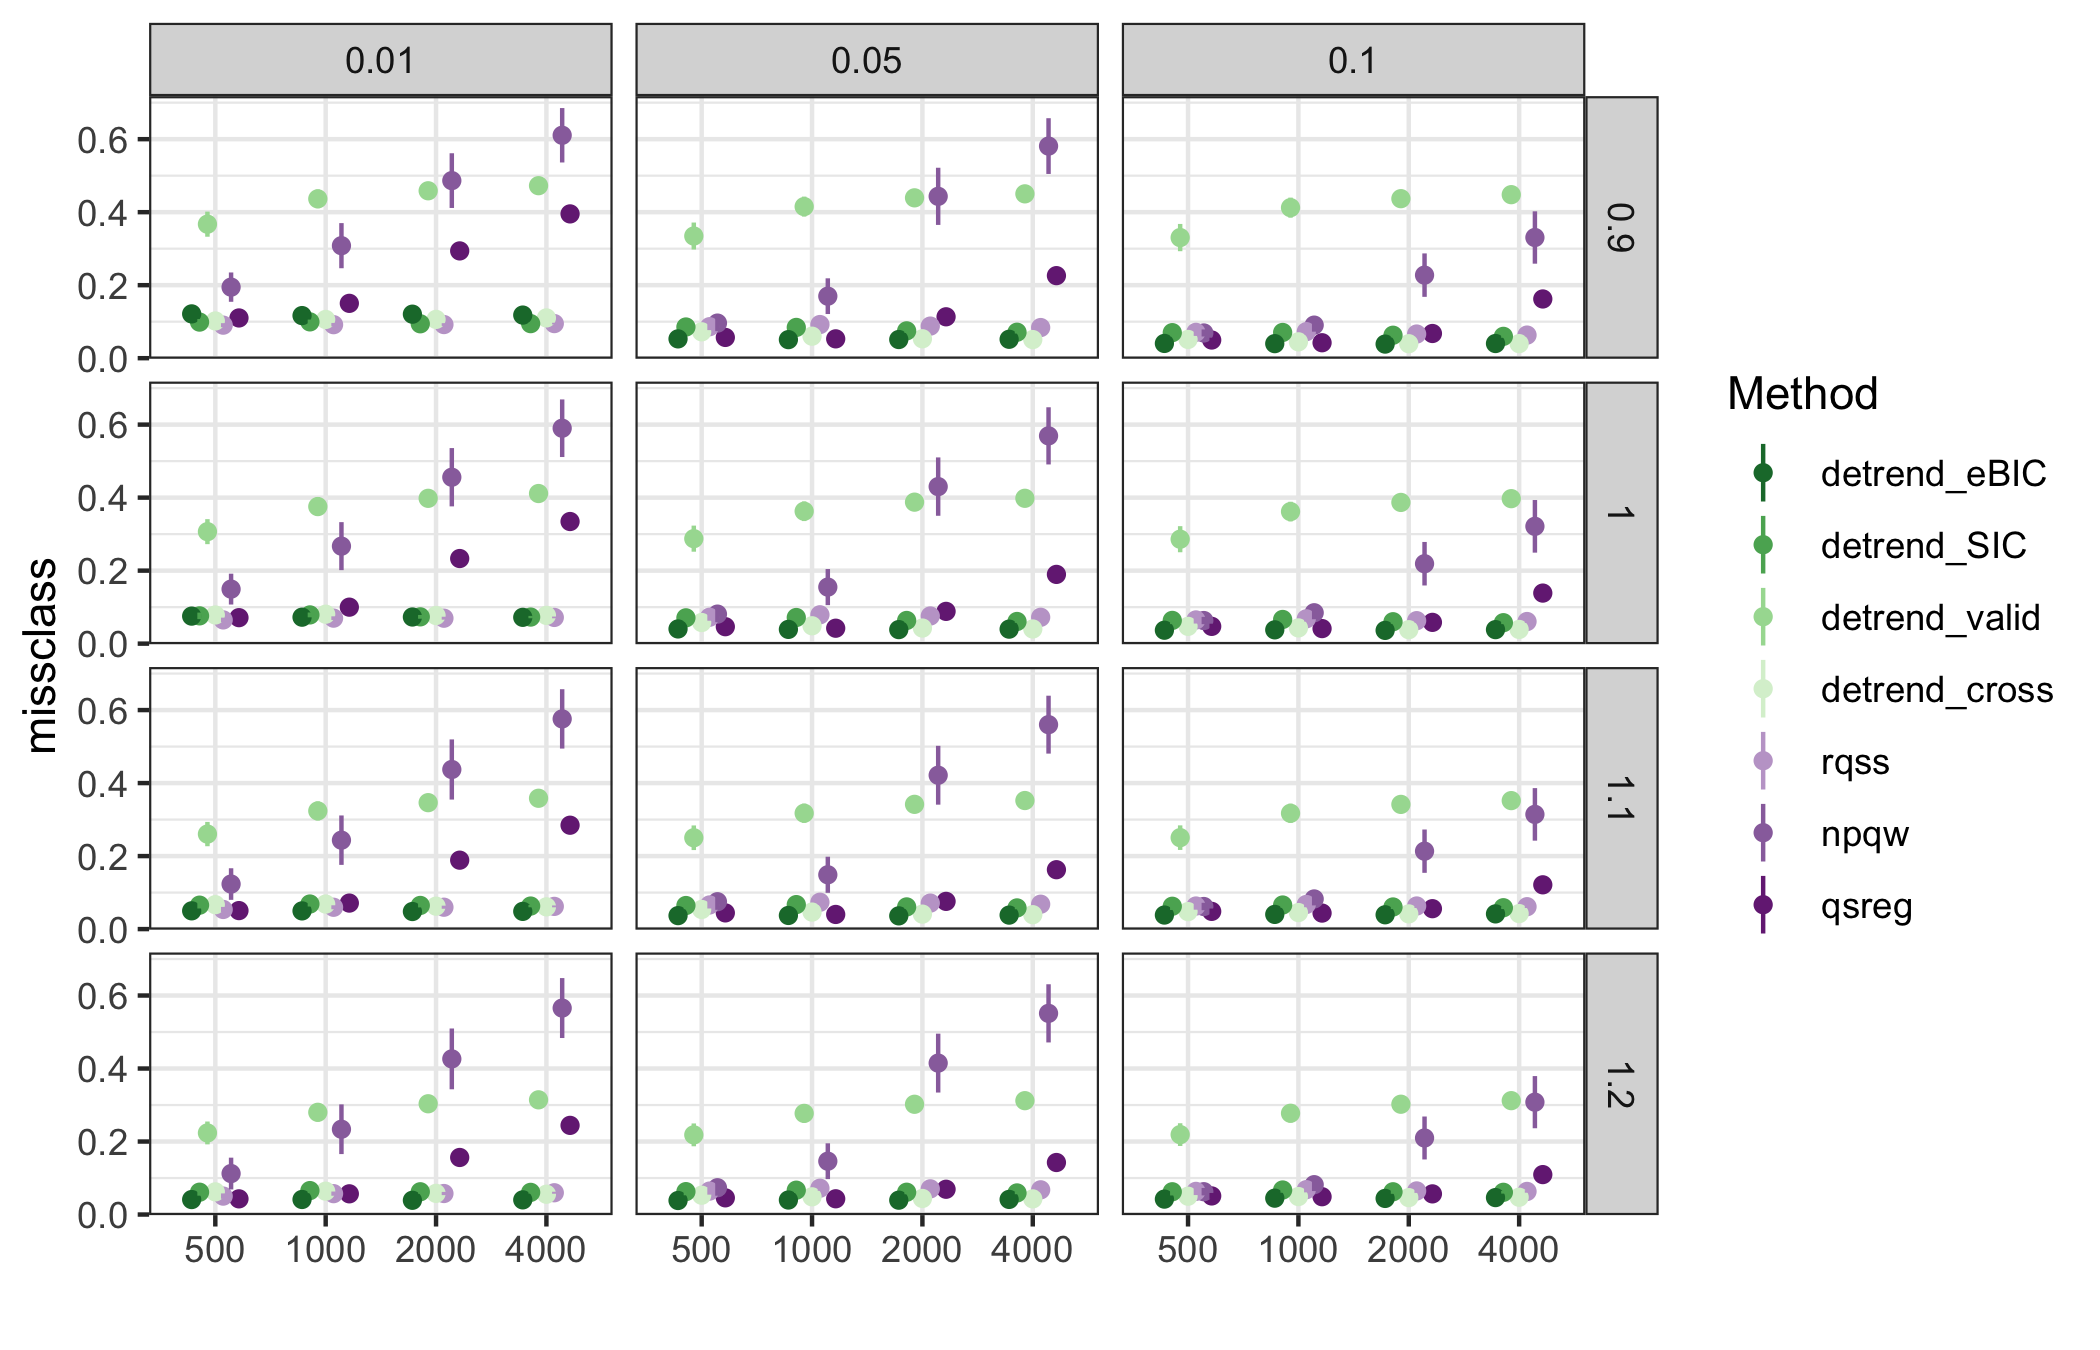
\includegraphics[width = \linewidth]{Figures/peaks_missclass.png}
	\end{figure}

	\section{Application Metrics}
	%latex.default(confusion %>% filter(crit == 3) %>% select(-crit),     file = "../Manuscript/short_confusion_detrend_MAD3.tex",     rowlabel = "", rowname = "", colheads = c("Method", "Quantile",         "0,0,0", "1,0,0", "0,1,0", "1,1,0", "1,0,0", "1,1,0",         "1,0,1", "1,1,1"), caption = "Confusion matrices for 3 SPod nodes after baseline \n      removal (n=5000). Node order is f, g, h. The threshold for the signal was \n      set as the median + 3*MAD.")%
\begin{table}[!tbp]
\caption{Confusion matrices for 3 SPod nodes after baseline 
      removal (n=5000). Node order is f, g, h. The threshold for the signal was 
      set as the median + 3*MAD.\label{confusion}} 
\begin{center}
\begin{tabular}{llrrrrrrrrr}
\hline\hline
\multicolumn{1}{l}{}&\multicolumn{1}{c}{Method}&\multicolumn{1}{c}{Quantile}&\multicolumn{1}{c}{0,0,0}&\multicolumn{1}{c}{1,0,0}&\multicolumn{1}{c}{0,1,0}&\multicolumn{1}{c}{1,1,0}&\multicolumn{1}{c}{1,0,0}&\multicolumn{1}{c}{1,1,0}&\multicolumn{1}{c}{1,0,1}&\multicolumn{1}{c}{1,1,1}\tabularnewline
\hline
&detrendr&$0.05$&$4571$&$16$&$37$&$105$&$14$&$16$&$ 6$&$235$\tabularnewline
&qsreg&$0.05$&$4575$&$37$&$35$&$121$&$11$&$ 4$&$14$&$203$\tabularnewline
&detrendr&$0.10$&$4567$&$20$&$41$&$107$&$14$&$16$&$ 6$&$229$\tabularnewline
&qsreg&$0.10$&$4580$&$42$&$42$&$ 97$&$ 7$&$ 5$&$30$&$197$\tabularnewline
&detrendr&$0.15$&$4574$&$21$&$34$&$106$&$14$&$16$&$ 6$&$229$\tabularnewline
&qsreg&$0.15$&$4599$&$46$&$33$&$ 91$&$11$&$ 3$&$34$&$183$\tabularnewline
\hline
\end{tabular}\end{center}
\end{table}

	%latex.default(confusion %>% filter(crit == 4) %>% select(-crit),     file = "../Manuscript/short_confusion_detrend_MAD4.tex",     rowlabel = "", rowname = "", colheads = c("Method", "Quantile",         "0,0,0", "1,0,0", "0,1,0", "1,1,0", "1,0,0", "1,1,0",         "1,0,1", "1,1,1"), caption = "Confusion matrices for 3 SPod nodes after baseline \n      removal (n=5000). Node order is f, g, h. The threshold for the signal was \n      set as the median + 4*MAD.")%
\begin{table}[!tbp]
\caption{Confusion matrices for 3 SPod nodes after baseline 
      removal (n=5000). Node order is f, g, h. The threshold for the signal was 
      set as the median + 4*MAD.\label{confusion}} 
\begin{center}
\begin{tabular}{llrrrrrrrrr}
\hline\hline
\multicolumn{1}{l}{}&\multicolumn{1}{c}{Method}&\multicolumn{1}{c}{Quantile}&\multicolumn{1}{c}{0,0,0}&\multicolumn{1}{c}{1,0,0}&\multicolumn{1}{c}{0,1,0}&\multicolumn{1}{c}{1,1,0}&\multicolumn{1}{c}{1,0,0}&\multicolumn{1}{c}{1,1,0}&\multicolumn{1}{c}{1,0,1}&\multicolumn{1}{c}{1,1,1}\tabularnewline
\hline
&detrendr&$0.05$&$4672$&$24$&$43$&$35$&$ 4$&$16$&$14$&$192$\tabularnewline
&qsreg&$0.05$&$4650$&$40$&$53$&$41$&$ 9$&$10$&$11$&$186$\tabularnewline
&detrendr&$0.10$&$4669$&$28$&$43$&$36$&$ 3$&$15$&$14$&$192$\tabularnewline
&qsreg&$0.10$&$4670$&$37$&$36$&$44$&$11$&$ 6$&$21$&$175$\tabularnewline
&detrendr&$0.15$&$4680$&$29$&$28$&$37$&$ 4$&$16$&$14$&$192$\tabularnewline
&qsreg&$0.15$&$4678$&$38$&$25$&$47$&$11$&$ 6$&$30$&$165$\tabularnewline
\hline
\end{tabular}\end{center}
\end{table}

	%latex.default(confusion %>% filter(crit == 5) %>% select(-crit),     file = "../Manuscript/short_confusion_detrend_MAD5.tex",     rowlabel = "", rowname = "", colheads = c("Method", "Quantile",         "0,0,0", "1,0,0", "0,1,0", "1,1,0", "1,0,0", "1,1,0",         "1,0,1", "1,1,1"), caption = "Confusion matrices for 3 SPod nodes after baseline \n      removal (n=7200). Node order is a, b, c. The threshold for the signal was \n      set as the median + 5*MAD.")%
\begin{table}[!tbp]
\caption{Confusion matrices for 3 SPod nodes after baseline 
      removal (n=7200). Node order is a, b, c. The threshold for the signal was 
      set as the median + 5*MAD.\label{confusion}} 
\begin{center}
\begin{tabular}{llrrrrrrrrr}
\hline\hline
\multicolumn{1}{l}{}&\multicolumn{1}{c}{Method}&\multicolumn{1}{c}{Quantile}&\multicolumn{1}{c}{0,0,0}&\multicolumn{1}{c}{1,0,0}&\multicolumn{1}{c}{0,1,0}&\multicolumn{1}{c}{1,1,0}&\multicolumn{1}{c}{1,0,0}&\multicolumn{1}{c}{1,1,0}&\multicolumn{1}{c}{1,0,1}&\multicolumn{1}{c}{1,1,1}\tabularnewline
\hline
&detrendr&$0.01$&$6672$&$171$&$61$&$ 83$&$27$&$1$&$40$&$145$\tabularnewline
&qsreg&$0.01$&$6526$&$150$&$84$&$208$&$19$&$2$&$27$&$184$\tabularnewline
&detrendr&$0.05$&$6723$&$ 71$&$64$&$146$&$26$&$1$&$22$&$147$\tabularnewline
&qsreg&$0.05$&$6478$&$247$&$78$&$206$&$ 1$&$3$&$13$&$174$\tabularnewline
&detrendr&$0.10$&$6717$&$ 83$&$60$&$143$&$17$&$1$&$21$&$158$\tabularnewline
&qsreg&$0.10$&$6468$&$292$&$71$&$203$&$ 1$&$3$&$15$&$147$\tabularnewline
\hline
\end{tabular}\end{center}
\end{table}


\end{document}